%%%%%%%%%%%%%%%%%%%%%%%%%%%%%%%%%%%%%%%%%%%%%%%%%%%%%%%%%%%%%%%%%%%%%%%%%%%%%%%%%%%
%% Projeto Final -- Protecao da SE Campus do Pici.
%% Tema UFC de Mauricio Moreira Neto: classe e preambulo originais preservados.
%% Roteiro: 10 slides, 13min30s estimados, sem sobreposicoes.
%% Compilar na pasta Slides: pdflatex, biber, pdflatex, pdflatex.
%%%%%%%%%%%%%%%%%%%%%%%%%%%%%%%%%%%%%%%%%%%%%%%%%%%%%%%%%%%%%%%%%%%%%%%%%%%%%%%%%%%
\documentclass{libs/ufc_format}
%%%%%%%%%%%%%%%%%%%%%%%%%%%%%%%%%%%%%%%%%%%%%%%%%%%%%%%%%%%%%%%%%%%%%
%% This file contains the packages that can be used in the beamer. %%
%%%%%%%%%%%%%%%%%%%%%%%%%%%%%%%%%%%%%%%%%%%%%%%%%%%%%%%%%%%%%%%%%%%%%
% Package to fonts family
\usepackage[T1]{fontenc}
% Package to accentuation
\usepackage[utf8]{inputenc}
% Package to Portuguese language
\usepackage[brazil]{babel}
% Package to Figures
\usepackage{graphicx}
% Package to the colors
\usepackage{color}
% Package to the colors
\usepackage{xcolor}
% Packages to math symbols and expressions
\usepackage{amsfonts, amssymb, amsmath}
% Package to multiple lines and columns in table
\usepackage{multirow, array} 
% Package to create pseudo-code
% For more detail of this package: http://linorg.usp.br/CTAN/macros/latex/contrib/algorithm2e/doc/algorithm2e.pdf
\usepackage{algorithm2e}
% Package to insert code
\usepackage{listings} 
\usepackage{keyval}
% Package to justify text
\usepackage[document]{ragged2e}
% Package to manage the bibliography
\usepackage[backend=biber, style=numeric, sorting=none]{biblatex}
% Package to facilities quotations
\usepackage{csquotes}
% Package to use multicols
\usepackage{multicol}
\addbibresource{../referencias.bib}
\usepackage{tikz}
\usetikzlibrary{arrows.meta}

% Foram mantidos formato, cores, fontes, fundo, cabecalho e rodape do modelo.
\setbeameroption{hide notes}
\newcommand{\fonteslide}[1]{%
    \par\smallskip{\scriptsize\color{blue_theme}Fonte: #1\par}}
\newcommand{\grafico}[3][36]{%
    \begin{center}
        \includegraphics[width=\linewidth,height=#3,keepaspectratio,
            trim=0 #1 0 0,clip]{../Imagens/#2}
    \end{center}}

\title[Proteção da SE Pici]{\texorpdfstring{%
    \Large\textbf{Coordenação e seletividade\\das proteções da SE Pici}}%
    {Coordenação e seletividade das proteções da SE Pici}}
\subtitle{Projeto Final --- Subestação 69--13,8~kV}
\author[Quinto, Marinho e Pinto]{\texorpdfstring{%
    \small Erika Oliveira Quinto\\
    Luiz Alberto Silva Sales Marinho\\
    Marcos Venicius de Oliveira Pinto}%
    {Erika Oliveira Quinto; Luiz Alberto Silva Sales Marinho; Marcos Venicius de Oliveira Pinto}}
\institute[UFC]{%
    \department{Departamento de Engenharia Elétrica}\\
    \ufc\\[0.15cm]
    {\small Proteção de Sistemas Elétricos de Potência\\
    Prof. Raimundo Furtado Sampaio}}
\date[2026.2]{2026.2}

\begin{document}

% 1/10 -- 00:30 -- acumulado 00:30.
\begin{frame}
    \maketitle
    \note{\textbf{Tempo sugerido: 30 segundos.}
    \begin{itemize}
        \item Apresentar a equipe e o sistema estudado.
        \item Anunciar o objetivo: coordenacao local e seletividade diferencial.
    \end{itemize}}
\end{frame}

% A marca inferior foi mantida na capa. Nos demais slides, foram mantidos
% a marca d'agua e o rodape, liberando a area das fontes e dos graficos.
\logo{}
\section{Sistema e TCs}

% 2/10 -- 01:30 -- acumulado 02:00.
\begin{frame}{Sistema estudado e premissas}
    \begin{center}
    \begin{tikzpicture}[x=1.25cm,y=1.05cm,
        every node/.style={font=\scriptsize},
        disjuntor/.style={draw,fill=white,minimum width=0.16cm,
            minimum height=0.22cm,inner sep=0pt},
        >=Latex]
        % Entrada e barramento de alta tensao.
        \draw[red,thick,->] (-0.25,1.45)--(1.55,1.45);
        \node[above] at (0.10,1.45) {Enel};
        \node[disjuntor,draw=red] at (0.85,1.45) {};
        \node[below] at (0.85,1.34) {12L1};
        \draw[red,very thick] (1.55,0.35)--(1.55,2.75);
        \node[above] at (1.55,2.75) {69 kV};

        % Unidade energizada.
        \draw[red,thick] (1.55,2.25)--(3.30,2.25);
        \node[disjuntor,draw=red] at (2.20,2.25) {};
        \node[above] at (2.20,2.38) {12T1};
        \draw[red,thick] (3.30,2.25) circle (0.18);
        \draw[blue_theme,thick] (3.57,2.25) circle (0.18);
        \node[above] at (3.44,2.55) {02T1};
        \node[below] at (3.44,1.99) {Em serviço};
        \draw[blue_theme,thick] (3.75,2.25)--(5.20,2.25);
        \node[disjuntor,draw=blue_theme] at (4.55,2.25) {};
        \node[above] at (4.55,2.38) {11T1};

        % Segunda unidade: reserva, sem paralelismo no cenario estudado.
        \draw[gray,dashed,thick] (1.55,0.75)--(3.30,0.75);
        \node[disjuntor,draw=gray] at (2.20,0.75) {};
        \node[above,text=gray] at (2.20,0.88) {12T2};
        \draw[gray,thick] (3.30,0.75) circle (0.18);
        \draw[gray,thick] (3.57,0.75) circle (0.18);
        \node[above,text=gray] at (3.44,1.05) {02T2};
        \node[below,text=gray] at (3.44,0.49) {Reserva};
        \draw[gray,dashed,thick] (3.75,0.75)--(5.20,0.75);
        \node[disjuntor,draw=gray] at (4.55,0.75) {};
        \node[above,text=gray] at (4.55,0.88) {11T2};

        % Barramento de media tensao e tres saidas radiais.
        \draw[blue_theme,very thick] (5.20,0.35)--(5.20,2.75);
        \node[above] at (5.20,2.75) {13,8 kV};
        \foreach \nivel/\saida in {2.25/1,1.50/2,0.75/3} {
            \draw[blue_theme,thick,->] (5.20,\nivel)--(7.15,\nivel);
            \node[disjuntor,draw=blue_theme] at (6.05,\nivel) {};
            \node[above] at (6.05,\nivel+0.12) {21L\saida};
        }
    \end{tikzpicture}
    \end{center}
    \begin{itemize}
        \item \textbf{Um transformador em serviço}; outro em reserva.
        \item 5/6,25~MVA; Dyn1; base ONAF de 6,25~MVA.
        \item Curtos fornecidos preservados; 12T1/12T2 incluídos.
    \end{itemize}
    \fonteslide{topologia simplificada do Projeto Final, caps.~1--2; roteiro de Sampaio (\citeyear{sampaio2026roteiro}).}
    \note{\textbf{Tempo sugerido: 1 minuto e 30 segundos.}
    \begin{itemize}
        \item Percorrer entrada, transformador em servico, geral MT e alimentadores.
        \item O segundo transformador nao foi considerado em paralelo.
        \item O esquema foi simplificado para apresentacao; as seccionadoras e funcoes constaram do unifilar completo.
    \end{itemize}}
\end{frame}

% 3/10 -- 01:30 -- acumulado 03:30.
\begin{frame}{TCs: critérios e relações adotadas}
    \begin{equation*}
        I_{p,\mathrm{TC}}\geq I_{\mathrm{carga}},\qquad
        20I_{p,\mathrm{TC}}\geq I_{\mathrm{cc},\max},\qquad
        V_s=\frac{I_{\mathrm{cc},\max}}{RTC}|Z_{\mathrm{ext}}|\leq200~\mathrm{V}
    \end{equation*}
    \begin{center}
    \small
    \renewcommand{\arraystretch}{1.35}
    \begin{tabular}{lrrrr}
        \hline
        \textbf{Aplicação} & \textbf{TC (A)} & \textbf{$I_{\mathrm{cc},\max}$ (kA)}
            & \textbf{$20I_p$ (kA)} & \textbf{$V_s$ (V)}\\
        \hline
        Entrada 12L1 & 1200/5 & 15,683 & 24,0 & 72,7\\
        12T1 e 12T2 & 800/5 & 15,683 & 16,0 & 109,0\\
        Gerais MT & 400/5 & 2,918 & 8,0 & 32,5\\
        Saídas e neutros & 200/5 & 2,918 & 4,0 & 65,0\\
        \hline
    \end{tabular}
    \end{center}
    \begin{itemize}
        \item Critérios aplicáveis atendidos nas hipóteses de cálculo.
        \item $FS=20$; $FT=1{,}2$; classe 10B200.
        \item Excitação e suportabilidade dos TCs a confirmar.
    \end{itemize}
    \fonteslide{Projeto Final, cap.~3, Tabelas de dimensionamento e especificação dos TCs.}
    \note{\textbf{Tempo sugerido: 1 minuto e 30 segundos.}
    \begin{itemize}
        \item Explicar os tres criterios e a diferenca entre corrente primaria do TC e relacao RTC.
        \item Destacar a revisao de alta: 1200/5 na entrada e 800/5 nos primarios.
        \item O limite de 16 kA dos TCs de 800/5 ficou proximo de 15,683 kA; nao houve comprovacao de estabilidade transitoria.
        \item Para o TC de neutro, nao foi informada corrente de carga para o primeiro criterio.
    \end{itemize}}
\end{frame}

\section{Sobrecorrente}

% 4/10 -- 01:30 -- acumulado 05:00.
\begin{frame}{Sobrecorrente: curva e ajustes de fase}
    \begin{equation*}
        t_{51}=\frac{13{,}5\,DT}{\min(I/I_p,30)-1}+t_a,
        \qquad I>I_p
    \end{equation*}
    \begin{center}
    \small
    \renewcommand{\arraystretch}{1.25}
    \begin{tabular}{lrrr}
        \hline
        \textbf{Proteção} & \textbf{$I_p$ primário (A)} & \textbf{$DT$} & \textbf{$t_a$ (s)}\\
        \hline
        Alimentadores 21L1--21L3 & 125,2 & 0,33 & 0,00\\
        Gerais MT: 11T1/11T2 & 328,0 & 0,38 & 0,00\\
        Primários AT: 12T1/12T2 & 65,6 & 0,68 & 0,00\\
        Entrada AT: 12L1 & 76,8 & 0,64 & 0,45\\
        \hline
    \end{tabular}
    \end{center}
    \begin{itemize}
        \item C2, IEC muito inversa; múltiplo limitado a 30.
        \item Margem local requerida: $\Delta t\geq0{,}40$~s.
        \item 50/50N desabilitadas nos gerais e na entrada.
    \end{itemize}
    \fonteslide{Projeto Final, cap.~4; Cysne (\citeyear{cysne2026protecao}); manual SEL-751 (\citeyear{sel2024sel751}).}
    \note{\textbf{Tempo sugerido: 1 minuto e 30 segundos.}
    \begin{itemize}
        \item Definir dial, corrente de partida e aditivo de tempo.
        \item Cada corrente da tabela foi referida ao proprio lado do transformador.
        \item O aditivo preservou a margem mesmo no patamar de multiplo maximo.
        \item No primario, 50 foi proposto em 998,4 A/0,05 s; o grupo normal nao cobriu a transferencia de toda a carga para uma saida.
    \end{itemize}}
\end{frame}

% 5/10 -- 01:30 -- acumulado 06:30.
\begin{frame}{Coordenação de fase na base de 13,8 kV}
    \grafico{01_coordenograma_fase_MT.pdf}{0.57\paperheight}
    \begin{itemize}
        \item 51 isolada em 2.882,7~A: \textbf{0,202 $\rightarrow$ 0,659 $\rightarrow$ 1,179 $\rightarrow$ 1,778~s}.
        \item Margem geral--primário na falta bifásica: aproximadamente \textbf{0,403~s}.
    \end{itemize}
    \fonteslide{Projeto Final, cap.~4; coordenograma elaborado pelos autores.}
    \note{\textbf{Tempo sugerido: 1 minuto e 30 segundos.}
    \begin{itemize}
        \item Ler as curvas da saida para a entrada, sempre na base de media tensao.
        \item Os tempos foram calculados para falta persistente proxima a saida; nao representaram quatro aberturas sucessivas.
        \item O estagio 50 da saida foi pre-ajuste de 2306,4 A/0,10 s, dependente dos religadores.
        \item O degrau 50 do primario foi mostrado em 4992 A, a direita do curto maximo de 2882,7 A.
        \item O dial de 0,68 foi definido pela verificacao bifasica Dyn1, separada da conversao trifasica do grafico.
    \end{itemize}}
\end{frame}

% 6/10 -- 01:15 -- acumulado 07:45.
\begin{frame}{Coordenação de neutro na base de 13,8 kV}
    \grafico{02_coordenograma_neutro_MT.pdf}{0.57\paperheight}
    \begin{itemize}
        \item 51N/51G em 2.918,4~A: \textbf{0,303 $\rightarrow$ 0,753 $\rightarrow$ 1,203~s}; margem de 0,45~s.
        \item Sequência zero bloqueada pelo triângulo no lado de 69~kV.
    \end{itemize}
    \fonteslide{Projeto Final, cap.~4; coordenograma elaborado pelos autores.}
    \note{\textbf{Tempo sugerido: 1 minuto e 15 segundos.}
    \begin{itemize}
        \item Associar 51N da saida, 51N do geral e 51G do neutro do transformador.
        \item Os limiares foram 24, 60 e 60 A; aditivos de 0, 0,45 e 0,90 s.
        \item Os 337 A refletidos na AT foram corrente de fase, nao corrente residual.
        \item 50N permaneceu pre-ajuste; 51NS dependeu do historico de desequilibrio.
    \end{itemize}}
\end{frame}

\section{Proteção diferencial}

% 7/10 -- 02:00 -- acumulado 09:45.
\begin{frame}{Proteção diferencial dos transformadores (87T)}
    \begin{center}
        \small\textbf{P642 sensível, 5 A}\quad
        TCs exclusivos: 800/5 AT e 400/5 MT
    \end{center}
    \begin{center}
        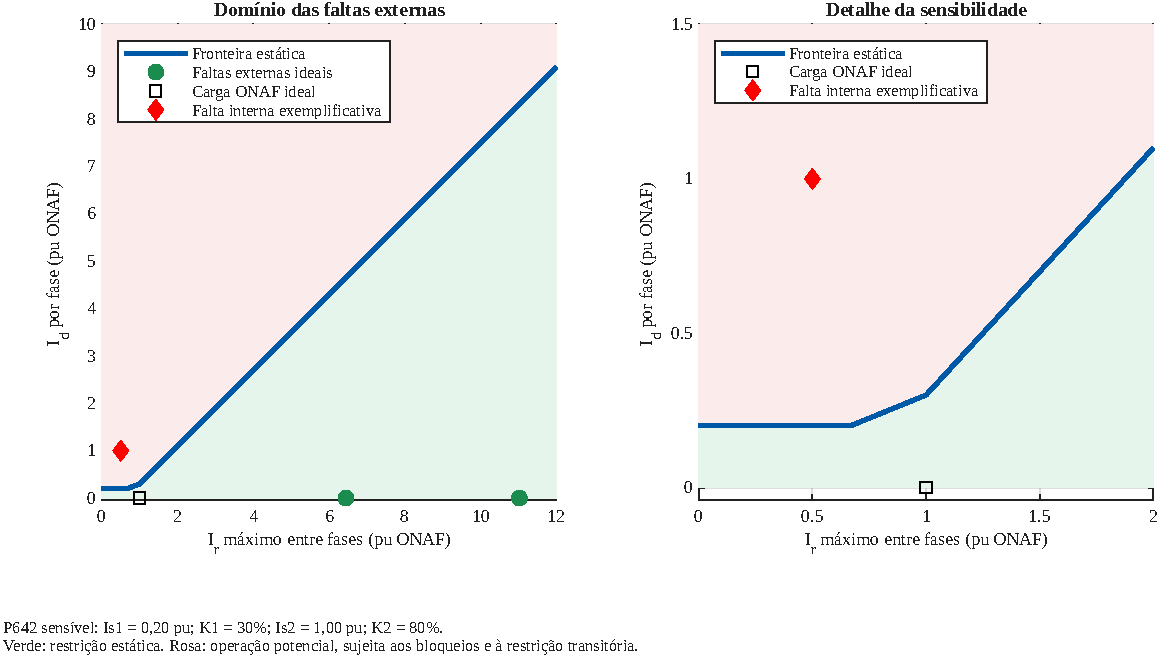
\includegraphics[width=\linewidth,height=0.39\paperheight,
            keepaspectratio,trim=0 35 0 0,clip]
            {../Imagens/08_caracteristica_diferencial.pdf}
    \end{center}
    \begin{equation*}
        I_{d,k}=|\underline J_{1k}+\underline J_{2k}|,\quad
        I_{r,k}=\frac{|\underline J_{1k}|+|\underline J_{2k}|}{2},\quad
        I_r=\max_k I_{r,k}
    \end{equation*}
    \begin{itemize}
        \item $I_{s1}=0{,}20$~pu; $K_1=30\%$; $I_{s2}=1$~pu; $K_2=80\%$.
        \item Dyn1; filtro de sequência zero; bloqueios harmônicos.
        \item Zona entre TCs AT/MT; abertura dos dois lados.
    \end{itemize}
    \fonteslide{Projeto Final, cap.~5; Cysne (\citeyear{cysne2026protecao}); manual P642 (\citeyear{gev2025p64x}).}
    \note{\textbf{Tempo sugerido: 2 minutos.}
    \begin{itemize}
        \item As grandezas J foram compensadas e normalizadas pela base ONAF de 6,25 MVA.
        \item Id e Ir foram definidos por fase; na fronteira comum foi utilizado o maior Ir entre fases.
        \item As faltas externas ideais ficaram com Id proximo de zero; o exemplo interno ficou acima da fronteira.
        \item A curva teve patamar ate 0,6667 pu e mudanca de declividade em 1 pu.
        \item O casamento AT de 15,2975 exigiu modulos sensiveis, proximo do limite de 15,38.
        \item Bloqueios H2/H5: 20/35 por cento; HS1: 32 pu de pico; HS2 desabilitado.
        \item A representacao estatica nao comprovou estabilidade transitoria dos TCs.
    \end{itemize}}
\end{frame}

\section{Retaguarda e interface}

% 8/10 -- 01:15 -- acumulado 11:00.
\begin{frame}{Falha de disjuntor e religamento}
    \grafico{07_diagrama_falha_disjuntor.pdf}{0.48\paperheight}
    \begin{itemize}
        \item 50BF: \textbf{0,25~s após comando de abertura (TR)}, supervisionada.
        \item 79: um religamento dos alimentadores; tempo morto de 10~s.
        \item Religamento bloqueado após 87T ou 50BF.
    \end{itemize}
    \fonteslide{Projeto Final, cap.~4; diagrama elaborado pelos autores.}
    \note{\textbf{Tempo sugerido: 1 minuto e 15 segundos.}
    \begin{itemize}
        \item A contagem de BF comecou no comando TR, nao no inicio da falta.
        \item Para TR em 0,100 s, BF em 0,350 s; para TR em 0,202 s, BF em 0,452 s.
        \item Foi pressuposta corrente persistente; comunicacao e abertura a montante nao foram somadas.
        \item A retaguarda da saida foi o geral em servico; a falha da entrada exigiu interface com a concessionaria.
        \item O religamento nao foi habilitado para os transformadores; os demais bloqueios constaram do relatorio.
    \end{itemize}}
\end{frame}

% 9/10 -- 01:30 -- acumulado 12:30.
\begin{frame}{Limite da seletividade com a concessionária}
    \grafico[23]{06_diagramas_tempo_barra_AT.pdf}{0.49\paperheight}
    \begin{alertblock}{Seletividade integral em 69 kV não demonstrada}
        \begin{itemize}
            \item Falta trifásica: 51 de Pici antes de 51 da entrada.
            \item 51N de Pici: estimativa analítica; distância a conferir.
        \end{itemize}
    \end{alertblock}
    \fonteslide{Projeto Final, cap.~4; OAP nº 046/2018, SED Pici II (\citeyear{enel2018oap}).}
    \note{\textbf{Tempo sugerido: 1 minuto e 30 segundos.}
    \begin{itemize}
        \item Comparar 0,134 s de Pici com 0,748 s da entrada para falta trifasica de barra.
        \item O tempo de Pici utilizou sua contribuicao de 15179,3 A; na entrada foram utilizados 15683,2 A.
        \item A referencia de neutro foi extrapolacao C2 com multiplo maior que 30, sem comprovacao do tempo efetivo.
        \item A diferencial nao cobriu a barra de 69 kV, externa a sua zona.
        \item A eliminacao pelo 50 do primario foi estimada entre 0,105 e 0,185 s; tampouco garantiu seletividade com Pici.
    \end{itemize}}
\end{frame}

\section{Conclusões}

% 10/10 -- 01:00 -- acumulado 13:30; reserva de 01:30 ate o limite de 15 min.
\begin{frame}{Conclusões e condições para implantação}
    \begin{exampleblock}{Resultados do estudo}
        \begin{itemize}
            \item TCs revisados: critérios de dimensionamento atendidos.
            \item Coordenação temporizada local: margens superiores a 0,40~s.
            \item Diferencial: separação dos casos ideais externos e interno.
        \end{itemize}
    \end{exampleblock}
    \begin{block}{Verificações que permaneceram necessárias}
        \begin{itemize}
            \item Curtos mínimos e religadores para liberação de 50/50N.
            \item Dados dos TCs, faixas dos IEDs e tempos reais de abertura.
            \item Coordenação com a concessionária e interface de disparo.
        \end{itemize}
    \end{block}
    \fonteslide{Projeto Final, caps.~6--7; bases documentais indicadas nos slides anteriores.}
    \note{\textbf{Tempo sugerido: 1 minuto.}
    \begin{itemize}
        \item Retomar o objetivo e os tres resultados, sem repetir todos os ajustes.
        \item Encerrar como proposta de estudo, dependente de verificacoes para implantacao.
        \item O roteiro totalizou 13min30s estimados, com reserva de 1min30s.
    \end{itemize}}
\end{frame}

\end{document}
